\section{From matching examples to certifying a computation}\label{sec:tasks}
\paragraph{What can one hidden layer achieve?}
For a positive real $L$, consider the shallow hinge network from Section~\ref{sec:matched} on $[-L,L]$. Its \emph{uniform error} on square is the supremum (least upper bound) of $|f(x)-x^2|$ over that interval. With $w$ hinges the graph has at most $w+1$ affine pieces. The smallest possible uniform error over real weights is exactly $L^2/[2(w+1)^2]$. To see the lower bound, take a segment of length $\ell$ on which the network is affine. For a function on its two endpoints and midpoint, the second difference is its endpoint sum minus twice its midpoint value. It is zero for an affine function and $\ell^2/2$ for square. If all three errors have magnitude at most $\eta$, their second difference has magnitude at most $4\eta$. At least one segment has length $2L/(w+1)$ or greater. Conversely, connect equally spaced square values by lines and shift the result down by half its largest interpolation error. This piecewise-affine function, or \emph{spline}, attains the bound. At $L=10$, a uniform tolerance of 0.01 first becomes possible at 70 hinges. A fixed absolute tolerance of $2^{-52}$ requires 474,531,328 hinges. Binary64 step sizes vary with the input and output magnitude.

A separate threshold holds for binary64 arithmetic. Limit all coefficient magnitudes to 128 and evaluate products and sums in the fixed order of Appendix~\ref{app:lattice-square}, rounding after each operation. Exactly 1,280 hinges (3,842 slots) are necessary and sufficient for correct square outputs on all 2,561 equally spaced sites in $[-10,10]$ at spacing $1/128$. The attaining network misses all 2,560 midpoints between those sites. Any network in this class that is correct on the entire binary64 interval must also be correct on the grid. The result gives a lower bound for that class and an exact minimum for the grid.

\paragraph{A sampled success, a shell proof, and an interval proof for square.}
For a contrast with shallow approximation, we constructed a multilayer perceptron (MLP), a sequence of affine maps and nonlinear activations, whose repeated tent-shaped map halves a grid spacing at each stage \cite{yarotsky2017error}. A correction path stores the small residual lost by rounding a subtraction. With 48 stages the corrected graph matched binary64 multiplication on 131,072 fresh outer inputs. On 304 outer inputs designed to put the exact square near a rounding boundary, it matched just 40. Figure~\ref{fig:prec} compares exactness with the correction present and removed. Appendix~\ref{app:square} specifies the construction.

\begin{figure}[htbp]\centering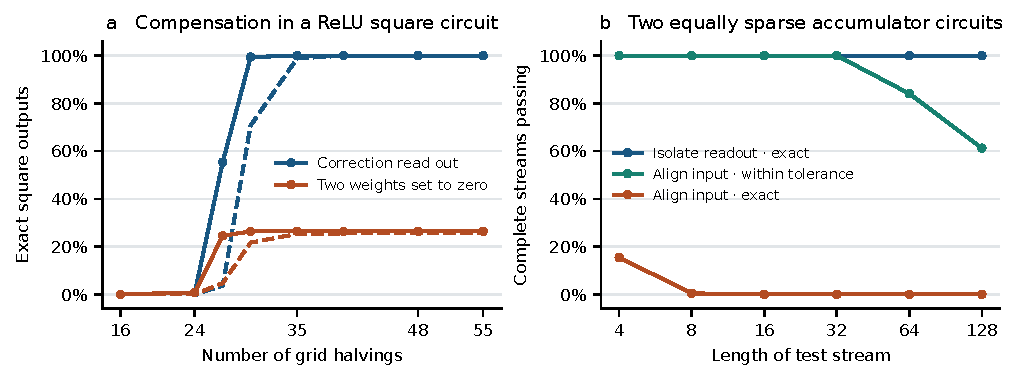
\includegraphics[width=\linewidth]{precision.pdf}
\caption{Two ways that a real-arithmetic identity can lose exact numerical agreement. Panel a varies the number of square refinements. Dashed lines use 4,096 central inputs, solid lines 8,192 outer inputs. The two networks differ only in whether the readout uses the accumulated rounding residual. Panel b compares two running-sum updates of width eight from Section~\ref{sec:front}. At each length, 64 initial networks are evaluated on the same 64 outer streams. Exact requires equality at every step. The tolerance curve requires $|\hat y-y|\le10^{-10}(1+|y|)$ at every step, where $y$ is the reference prefix sum and $\hat y$ the predicted sum.}\label{fig:prec}
\end{figure}

In a different experiment Astra received the square rule and could choose both the connections and coefficients of an affine/ReLU graph. It received no rounding-boundary failures before answering. One of three first replies computed the correctly rounded square for \emph{every} binary64 input in the two outer intervals using 2,543 input-dependent operations. Its graph extracts the significant digits, forms their integer product in three fixed-size pieces, and retains enough discarded information to round once at the end. Appendix~\ref{app:literal-square-certificate} proves the claim and gives an interior counterexample. We then added a rounding path for \emph{subnormal} results, the small-magnitude values below the smallest positive normal number in magnitude, with uniform spacing $2^{-1074}$. The engineered WSP graph uses 3,352 operations and is correct on all binary64 inputs in $[-10,10]$ (Appendix~\ref{app:fullsquare}). Both size counts are achieved upper bounds. The minimum for a deep graph remains open.

\paragraph{Sine, self-power and hyperbolic tangent.}
Our engineered WSP circuits for sine and positive self-power use affine operations and ReLUs. Their respective 500 and 1,352 stored coefficient words are individually addressable binary64 values. At inference both circuits matched the correctly rounded mathematical target on 32,768 fresh outer inputs, giving zero RMSE on those draws. We also used CORE-MATH, a project publishing difficult inputs for correctly rounded mathematical functions. The sine circuit missed 12 of 30,326 hard cases in its design interval $[-16,16]$ and one of the 1,884 in the requested shell. The self-power circuit missed 450 of 896 inputs chosen near output rounding boundaries just below one. Each miss was one adjacent representable value. The WSP hyperbolic tangent matched all 60,574 signed CORE-MATH cases in $[-10,10]$. Appendices~\ref{app:smooth-circuits} and \ref{app:relu-tanh} give run sizes and raw errors. On the deployed self-power and hyperbolic-tangent graphs, none of three BP fits per graph came within one ULP on an outer example after 100 Adam updates. The best of the three hyperbolic-tangent fits still achieved outer RMSE about 0.095. Tested hard cases establish measured accuracy for these circuits. Global correctness of their last output digit remains open.

\paragraph{Sorting without perturbing an input.}
For each ordering of four distinct real inputs, sorting applies a different permutation of the four coordinates. On the region corresponding to that ordering the derivative matrix (Jacobian) is the associated permutation matrix. A feedforward affine/ReLU graph with $g$ scalar ReLUs has at most $2^g$ patterns of active units and therefore at most $2^g$ distinct Jacobians on open regions. As $4!=24$, at least five gates are necessary. Five suffice over the reals: a \emph{comparator} sorts a pair $(a,b)$ by forming $t=R(a-b)$ and returning $(a-t,b+t)$. Applying it to five prescribed pairs sorts four inputs \cite{batcher1968sorting}. Subtracting a rounded difference can perturb one operand in binary64. In the fixed-schedule outer test this WSP sorter matched 1,105 of 2,048 lists with RMSE $5.12\times10^{-16}$.

A different comparator uses 13 ReLUs to select and transmit an original operand. It has 50 stored coefficients shared across comparisons. Sorting four inputs uses 65 ReLU executions, with 250 coefficient uses. Appendix~\ref{app:sort} proves that the comparator returns both original numerical values in order for every binary64 pair in $[-10,10]^2$, with signed zeros treated as equal. The resulting four-item WSP sorter had zero RMSE on the outer test. Five matched BP fits had median RMSE 4.35 and zero exact outer lists at the median. This gives a binary64 upper bound on gate count. The five-gate lower bound above concerns real arithmetic.
